\documentclass[11pt]{report}

\usepackage[utf8]{inputenc}

%%% PAGE DIMENSIONS
\usepackage{geometry} % to change the page dimensions
\geometry{a4paper} % or letterpaper (US) or a5paper or....
\geometry{top=2.5cm}
\geometry{right=2.5cm}
\geometry{bottom=2cm}
\geometry{left=2.5cm}

\usepackage{graphicx}
\usepackage{amsmath}
\usepackage{amssymb}
\usepackage{csquotes}
\usepackage{hyperref}
\usepackage[nonumberlist]{glossaries}  
\usepackage{titlesec}
\usepackage[normalem]{ulem}
\usepackage{nameref}
\usepackage{pdfpages}
\usepackage{framed}
\usepackage[ngerman]{babel}
\usepackage[T1]{fontenc}
\usepackage{booktabs}
\usepackage{array}
\usepackage{paralist}
\usepackage{verbatim}
\usepackage{subfig}
\usepackage{multicol}
\usepackage{caption}
\usepackage{footnote}
\usepackage{listings}
\usepackage{color}
\usepackage{selinput}
\usepackage{float}
\SelectInputMappings{
	adieresis={ä},
	germandbls={ß}
}
\usepackage{babel}
\usepackage{ulem}
\usepackage{placeins}


% Spezialpakete

\usepackage{tikz}
% TikZ-Bibliotheken
\usetikzlibrary{arrows}
\usetikzlibrary{shapes}
\usetikzlibrary{decorations.pathmorphing}
\usetikzlibrary{decorations.pathreplacing}
\usetikzlibrary{decorations.shapes}
\usetikzlibrary{decorations.text}


%%% HEADERS & FOOTERS
\usepackage{fancyhdr}
\pagestyle{fancy}
\renewcommand{\headrulewidth}{0pt}
\lhead{}\chead{}\rhead{}
\lfoot{}\cfoot{\thepage}\rfoot{}
\usepackage[default,osfigures,scale=0.95]{opensans} %% 
\usepackage[T1]{fontenc}

%%% ToC (table of contents) APPEARANCE
\usepackage[nottoc,notlof,notlot]{tocbibind}
\usepackage[titles,subfigure]{tocloft}
\renewcommand{\cftsecfont}{\rmfamily\mdseries\upshape}
\renewcommand{\cftsecpagefont}{\rmfamily\mdseries\upshape}

\newcommand{\HRule}[1]{\rule{\linewidth}{#1}} 	% Horizontal rule

%%%%%%%%%%%%%%%%%%%%%%%%%%%%%%
\titleformat{\chapter}{\normalfont\huge}{\thechapter.}{20pt}{\huge\it}

\begin{document}
	\begin{titlepage}
		\begin{center}
			\textsc{\Large Spezifikation}\\
			
			% Title
			{ \huge \bfseries Flexible ALU \\[0.4cm] }
			\HRule{0.5pt} \\[2.5cm]			
		\end{center}
		
		\begin{table}[h]
			\centering
			\begin{tabular}{l|l|l}
				\multicolumn{1}{c|}{\Large \textbf{  Version  }} & \multicolumn{1}{c|}{\Large \textbf{  Bearbeiter  }} & \multicolumn{1}{c}{\Large \textbf{  Neuerung  }} \\ \hline
				\multicolumn{1}{c|}{1.0}              & \multicolumn{1}{c|}{}                    & \multicolumn{1}{c}{}                  \\
				&                                          &                                       \\
				&                                          &                                      
			\end{tabular}
		\end{table}
		
		\vfill
		\begin{flushright}
			HFI414\\
			Q1 2016\\
			Torben Voltmer\\
			Sarah Wöckener\\
		\end{flushright}
	\end{titlepage}
	%%%%%%%%%%%%%%%%%%%%%%%%%%%%%%%%%%%
	\tableofcontents
	
	\pagebreak
	%%%%%%%%%%%%%%%%%%%%%%%%%%%%%%%%%%%
	
	\chapter{Preambel}
	
	\chapter{Datenblatt}
	
	\section{Einsatzbereich}
	Diese flexible ALU kann als arithmetisch/logische Einheit in einem Mikroprozessor verwendet werden.
	\colorbox{red}{Durch zwei in Microcode realisierbare Befehle...}
	
	\section{Features}
	\begin{itemize}
		\item Addition und Subtraktion zweier 4 Bit Operanden erzeugen ein 5 Bit langes Ergebnis.
		\item Multiplikation zweier 4 Bit Operanden erzeugt ein 8 Bit langes Ergebnis.
		\item Native Befehle werden in 2 Takten verarbeitet (Microcode ausgeschlossen).
		\item \colorbox{red}{2 Akkumulator Register für Microcode.}
		\item Für Microcode kann ein Barrel-Shifter verwendet werden.
		\item Alle Ein- und Ausgänge werden in Registern erhalten.
	\end{itemize}
	
	\section{Funktion}
	\begin{table}[h]
		\centering
		\label{codierungstabelle}
		\begin{tabular}{|lll|l|}
			\hline
			\multicolumn{3}{|c|}{CMD}                            & \multicolumn{1}{c|}{}             \\
			\multicolumn{1}{|l|}{2} & \multicolumn{1}{l|}{1} & 0 & Arithmetisch/logischer Ausdruck \\ \hline
			0                       & 0                      & 0 & AND                               \\ \hline
			0                       & 0                      & 1 & OR                                \\ \hline
			0                       & 1                      & 0 & NOT                               \\ \hline
			0                       & 1                      & 1 & ADD                               \\ \hline
			1                       & 0                      & 0 & SUB                               \\ \hline
			1                       & 0                      & 1 & MUL                               \\ \hline
			1                       & 1                      & 0 & MC0                               \\ \hline
			1                       & 1                      & 1 & MC1                               \\ \hline
		\end{tabular}
		\caption{Befehls-Codierung}
	\end{table}
	\FloatBarrier
	Für die Liste aller Port siehe Seite \pageref{portliste} Abbildung \ref{portliste}.\\
	\begin{itemize}
		\item Der Befehl \underline{AND} legt das Ergebnis an den ersten Operanden A0..3 an.
		\item Der Befehl \underline{OR} legt das Ergebnis an den ersten Operanden A0..3 an.
		\item Der Befehl \underline{NOT} negiert die Bits der Ports A0..3 und legt das Ergebnis an diesen wieder an.
		\item Der Befehl \underline{ADD} addiert A0..3 und B0..3 und legt das Ergebnis an A0..3 an. Tritt bei der Berechnung ein Carry auf, wird dieser in B0 dargestellt und das Ergebnis ist somit 5 Bit lang.
		\item Der Befehl \underline{SUB} subtrahiert B0..3 von A0..3 und gibt das Ergebnis an A0..3 aus. Dieses Ergebnis befindet sich im 2er-Komplement!
		\item Der Befehl \underline{MUL} multipliziert A0..3 und B0..3 und legt das 8 Bit breite Ergebnis an diese Ports an.
		\item Bei den Befehlen \underline{MC0} und \underline{MC1} handelt es sich zum Zeitpunkt der Anfertigung des Datenblattes um keine konkreten Befehle. Diese werden mit Hilfe von Microcode implementiert. Eine Erklärung dazu erhalten Sie im Spezifikationsteil dieses Dokumentes in Kapitel \ref{microcode_erklaerung}.
	\end{itemize}
	
	\section{Blockschaltbild}
	\begin{figure}[h]
		\begin{center}
			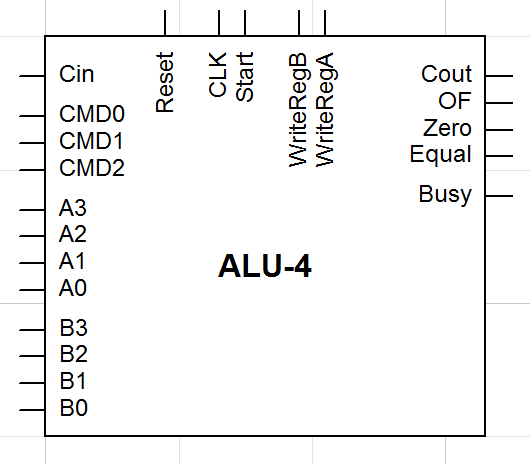
\includegraphics[]{aeusseresBlockschaltbild}
			\label{aeusseresBlockschaltbild}
			\caption{Äußeres Blockschaltbild}\label{aeusseresBlockschaltbild}
		\end{center}
	\end{figure}
	\FloatBarrier
	Für detaillierte Informationen zu Ein- und Ausgängen siehe Tabelle \ref{portliste}.\\
	
	\section{Schnittstellen}
	\begin{table}[h]
		\centering
		\begin{tabular}{|l|l|p{11cm}|}
			\hline
			Port      & Typ           & Funktion                                                                                                                                                                                                       \\ \hline\hline
			Cin       & Input         & Carry-In für ADD und SUB                                                                                                                                                                                       \\ \hline
			WriteRegA & Input         & Wenn 1, wird Operand 1 in Register A geschrieben (solange die Arbitrierung außen liegt).                                                                                                                       \\ \hline
			WriteRegB & Input         & Wenn 1, wird Operand 2 in Register B geschrieben (solange die Arbitrierung außen liegt).                                                                                                                       \\ \hline
			Reset     & Input         & Register werden asynchron (ohne Taktflanke) zurückgesetzt.                                                                                                                                                     \\ \hline
			Start     & Input         & Die Operation wird mit den angelegten Operanden durchgeführt.                                                                                                                                                  \\ \hline
			CLK       & Input         & Takt.                                                                                                                                                                                                          \\ \hline
			CMD0..2   & Input         & Auswahl des Befehls. Codierung siehe Tabelle \ref{codierungstabelle}.\\ \hline
			A0..3     & Bidirektional & IN: Operand 1 wird mit WriteRegA angelegt. OUT: Ist Busy 0, liegt hier das Ergebnis der Berechnung an. Die Subtraktion liefert das 2er-Komplement. Multiplikation liefert hier das low-nibble des Ergebnisses. \\ \hline
			B0..3     & Bidirektional & IN: Operand 2 wird mit WriteRegB angelegt. OUT: Wird Busy 0, liegt hier 0 an, die Multiplikation liefert hier das high Nibble des Ergebnisses.                                                                 \\ \hline
			Busy      & Output        & Ist 1, solange die ALU arbeitet. Wird Busy 0, liegt das Ergebnis an A0..3 und B0..3 an. Die Arbitrierung von RegA und RegB liegt außen, solange Busy = 0 ist.                                                    \\ \hline
			OF (Flag)        & Output        & OF ist 1, wenn die letzten beiden Übertragsbits ungleich sind und somit ein Overflow auftritt.                                                                                                                 \\ \hline
			Zero (Flag)     & Output        & Zero ist 1, wenn alle Ergebnisbits 0 sind.                                                                                                                                                                     \\ \hline
			Equal (Flag)     & Output        & Equal ist 1, wenn die Operanden A und B bitweise gleich sind.                                                                                                                                                  \\ \hline
			Cout (Flag)      & Output        & Carry out. Tritt während der Berechnung von ADD oder SUB ein Übertrag über die letzte Bitstelle auf, wird Cout 1 und kann weiter behandelt werden.                                                             \\ \hline
		\end{tabular}
		\caption{Liste aller Ports} \label{portliste}
	\end{table}
	\FloatBarrier
	Tabelle \ref{flagtable} können Sie Informationen zur Relevanz der ausgegebenen Flags entehmen.\\
	
	\begin{table}[h]
		\centering
		\begin{tabular}{l|l|p{8cm}}
			Flag  & relevant für                       & Auswirkung   \\ \hline
			Cout  & Addition, Subtraktion              & Das Bit ist Repräsentant für einen in das nächste Nibble übergehenden Carry und muss zur Ermittlung des Ergebnisses berücksichtigt werden.\\
			OF    & Subtraktion                     & Die Subtraktion liefert OF = 1, wenn ein Carry auftritt und die MSBits der Operanden im Zweierkomplement gleich sind. \\
		\end{tabular}
		\caption{Flag-Relevanz} \label{flagtable}
	\end{table}
	\FloatBarrier
	Das Ergebnis keiner Funktion ist funktional von Equal und Zero abhängig.
	
	\section{Gate-Count}
	Für eine detaillierte Angabe der Gatteräquivalente siehe Abbildung \ref{gatecount} auf Seite \pageref{gatecount}.
	\begin{table}[h]
		\small
		\centering
		\label{gatecount}
		\begin{tabular}{llll}
			\hline
			Typ                                          & Gatteräquivalente          & Anzahl                  & Summe                      \\ \hline\hline
			\multicolumn{1}{|l}{Gatter}                  &                            &                         & \multicolumn{1}{l|}{}      \\ \hline
			\multicolumn{1}{|l|}{AND2}                   & \multicolumn{1}{l|}{1,5}   & \multicolumn{1}{l|}{65} & \multicolumn{1}{l|}{97,5}  \\ \hline
			\multicolumn{1}{|l|}{AND3}                   & \multicolumn{1}{l|}{2}     & \multicolumn{1}{l|}{13} & \multicolumn{1}{l|}{26}    \\ \hline
			\multicolumn{1}{|l|}{AND4}                   & \multicolumn{1}{l|}{2,5}   & \multicolumn{1}{l|}{12} & \multicolumn{1}{l|}{30}    \\ \hline
			\multicolumn{1}{|l|}{AND5}                   & \multicolumn{1}{l|}{3}     & \multicolumn{1}{l|}{4}  & \multicolumn{1}{l|}{12}    \\ \hline
			\multicolumn{1}{|l|}{Inv}                    & \multicolumn{1}{l|}{0,5}   & \multicolumn{1}{l|}{11} & \multicolumn{1}{l|}{5,5}   \\ \hline
			\multicolumn{1}{|l|}{Mult2:1}                & \multicolumn{1}{l|}{3}     & \multicolumn{1}{l|}{28} & \multicolumn{1}{l|}{84}    \\ \hline
			\multicolumn{1}{|l|}{Mult4:1}                & \multicolumn{1}{l|}{7}     & \multicolumn{1}{l|}{0}  & \multicolumn{1}{l|}{0}     \\ \hline
			\multicolumn{1}{|l|}{Mult8:1}                & \multicolumn{1}{l|}{16}    & \multicolumn{1}{l|}{9}  & \multicolumn{1}{l|}{144}   \\ \hline
			\multicolumn{1}{|l|}{NAND2}                  & \multicolumn{1}{l|}{1}     & \multicolumn{1}{l|}{6}  & \multicolumn{1}{l|}{6}     \\ \hline
			\multicolumn{1}{|l|}{NAND3}                  & \multicolumn{1}{l|}{1,5}   & \multicolumn{1}{l|}{0}  & \multicolumn{1}{l|}{0}     \\ \hline
			\multicolumn{1}{|l|}{NAND4}                  & \multicolumn{1}{l|}{2}     & \multicolumn{1}{l|}{0}  & \multicolumn{1}{l|}{0}     \\ \hline
			\multicolumn{1}{|l|}{NAND6}                  & \multicolumn{1}{l|}{4,5}   & \multicolumn{1}{l|}{0}  & \multicolumn{1}{l|}{0}     \\ \hline
			\multicolumn{1}{|l|}{NAND8}                  & \multicolumn{1}{l|}{5,5}   & \multicolumn{1}{l|}{0}  & \multicolumn{1}{l|}{0}     \\ \hline
			\multicolumn{1}{|l|}{NOR2}                   & \multicolumn{1}{l|}{1}     & \multicolumn{1}{l|}{0}  & \multicolumn{1}{l|}{0}     \\ \hline
			\multicolumn{1}{|l|}{NOR3}                   & \multicolumn{1}{l|}{1,5}   & \multicolumn{1}{l|}{0}  & \multicolumn{1}{l|}{0}     \\ \hline
			\multicolumn{1}{|l|}{NOR4}                   & \multicolumn{1}{l|}{2}     & \multicolumn{1}{l|}{0}  & \multicolumn{1}{l|}{0}     \\ \hline
			\multicolumn{1}{|l|}{OR2}                    & \multicolumn{1}{l|}{1,5}   & \multicolumn{1}{l|}{21} & \multicolumn{1}{l|}{31,5}  \\ \hline
			\multicolumn{1}{|l|}{OR3}                    & \multicolumn{1}{l|}{2}     & \multicolumn{1}{l|}{4}  & \multicolumn{1}{l|}{8}     \\ \hline
			\multicolumn{1}{|l|}{OR4}                    & \multicolumn{1}{l|}{2,5}   & \multicolumn{1}{l|}{9}  & \multicolumn{1}{l|}{22,5}  \\ \hline
			\multicolumn{1}{|l|}{OR5}                    & \multicolumn{1}{l|}{3}     & \multicolumn{1}{l|}{4}  & \multicolumn{1}{l|}{12}    \\ \hline
			\multicolumn{1}{|l|}{XNOR2}                  & \multicolumn{1}{l|}{3}     & \multicolumn{1}{l|}{0}  & \multicolumn{1}{l|}{0}     \\ \hline
			\multicolumn{1}{|l|}{XOR2}                   & \multicolumn{1}{l|}{3}     & \multicolumn{1}{l|}{32} & \multicolumn{1}{l|}{96}    \\ \hline
			\multicolumn{1}{|l}{Speicher (Angabe / bit)} &                            &                         & \multicolumn{1}{l|}{}      \\ \hline
			\multicolumn{1}{|l|}{DFF}                    & \multicolumn{1}{l|}{7}     & \multicolumn{1}{l|}{4}  & \multicolumn{1}{l|}{28}    \\ \hline
			\multicolumn{1}{|l|}{DFF-R}                  & \multicolumn{1}{l|}{8}     & \multicolumn{1}{l|}{0}  & \multicolumn{1}{l|}{0}     \\ \hline
			\multicolumn{1}{|l|}{DFF-S}                  & \multicolumn{1}{l|}{8}     & \multicolumn{1}{l|}{0}  & \multicolumn{1}{l|}{0}     \\ \hline
			\multicolumn{1}{|l|}{DFF-SR}                 & \multicolumn{1}{l|}{9}     & \multicolumn{1}{l|}{0}  & \multicolumn{1}{l|}{0}     \\ \hline
			\multicolumn{1}{|l|}{DRAM}                   & \multicolumn{1}{l|}{5}     & \multicolumn{1}{l|}{0}  & \multicolumn{1}{l|}{0}     \\ \hline
			\multicolumn{1}{|l|}{DRAM (o. Anst.)}        & \multicolumn{1}{l|}{0,25}  & \multicolumn{1}{l|}{0}  & \multicolumn{1}{l|}{0}     \\ \hline
			\multicolumn{1}{|l|}{SRAM}                   & \multicolumn{1}{l|}{7,5}   & \multicolumn{1}{l|}{0}  & \multicolumn{1}{l|}{0}     \\ \hline
			\multicolumn{1}{|l|}{SRAM (o. Anst.)}        & \multicolumn{1}{l|}{1}     & \multicolumn{1}{l|}{0}  & \multicolumn{1}{l|}{0}     \\ \hline
			\multicolumn{1}{|l|}{Buffer4}                & \multicolumn{1}{l|}{4}     & \multicolumn{1}{l|}{19} & \multicolumn{1}{l|}{76}    \\ \hline
			\multicolumn{1}{|l|}{74\_181}                & \multicolumn{1}{l|}{108,5} & \multicolumn{1}{l|}{1}  & \multicolumn{1}{l|}{108,5} \\ \hline\hline
			Gesamtsumme:                                 &                            &                         & 787,5                      \\ \hline
		\end{tabular}
		\caption{Gatteräquivalente}\label{gatecount}
	\end{table}
	\FloatBarrier
	
	\section{Timing-Diagramm}
	\begin{figure}[htbp]
		\begin{center}
			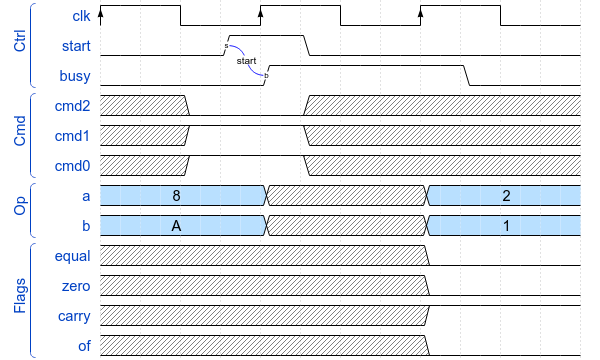
\includegraphics[width=\textwidth]{native_timing}
			\label{native_timing}
			\caption{Timingdiagramm der Addition}\label{native_timing}
		\end{center}
	\end{figure}
	\FloatBarrier
	\begin{figure}[htbp]
		\begin{center}
			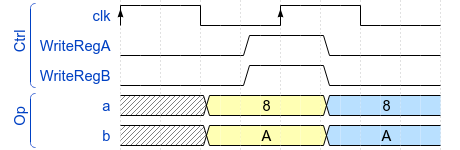
\includegraphics[width=\textwidth]{write_reg_timing}
			\label{write_reg_timing}
			\caption{Timingdiagramm des Registerschreibvorgangs}\label{write_reg_timing}
		\end{center}
	\end{figure}
	\FloatBarrier
	
	\section{Leistungsabschätzung}
	watt pro gatter pro mhz als energieverbrauch
	
	
	\chapter{Spezifikation}
	
	\section{Register}
	\subsection{RegA}
	Register für Operand A und das low-nibble des Ergebnisses.
	Es handelt sich um ein Bi-Reg-4.
	Die Arbitrierung des Registers liegt intern, solange Busy = 0 ist.
	Das Ergebnis liegt am Ausgang an, sobald Busy = 0 wird.
	
	\subsection{RegB}
	Register für Operand B und das high-nibble des Ergebnisses.
	Es handelt sich um ein Bi-Reg-4.
	Die Arbitrierung des Registers liegt intern, solange Busy = 0 ist.
	Das Ergebnis liegt am Ausgang an, sobald Busy = 0 wird.
	
	\subsection{AccuA}
	Akkumulatorregister für das low-nibble des Ergebnisses.
	Es handelt sich um ein Uni-Reg-4.
	Die Ausgänge des Registers können als Operand A verwendet werden.
	
	\subsection{AccuB}
	Akkumulatorregister für das high-nibble des Ergebnisses.
	Es handelt sich um ein Uni-Reg-4.
	Die Ausgänge des Registers können als Operand B verwendet werden.
	
	\subsection{CMD}
	Register für den Befehlscode.
	Es handelt sich um ein Uni-Reg-3. Wir geschrieben sobald Start = 1 gesetzt wird.
	
	\subsection{Flags}
	Register für die Flags.
	Es handelt sich um ein Uni-Reg-4.
	Die Flags liegen am Ausgang an, sobald Busy = 0 wird.
	
	
	\section{Modul-Beschreibung}
	\subsection{74181}
	Die 74181 dient zur Berechnung aller nativen ALU-Befehle außer der Multiplikation.
	
	\subsection{MUL-4}
	Ein 4x4 Bit Hardware-Multiplizierer mit 8 Bit Ausgang.
	
	\subsection{Barrel-Shifter-8}
	Ein 8-Bit Barrel-Shifter, der links/rechts rotieren/schieben um  0-7 Bit kann.
	\subsection{Bi-Reg-n}
	
	\subsection{Uni-Reg-n}
	Ein 
	
	\subsection{MUX-nxm}
	Multiplexer zum Schalten von n Signalquellen mit je m Bits.
	
	\subsection{MC-PROM}
	\label{microcode_erklaerung}
	\subsubsection{Programmierung}
	
	\section{Detailblockschaltbild}
	\begin{figure}[htbp]
		\begin{center}
			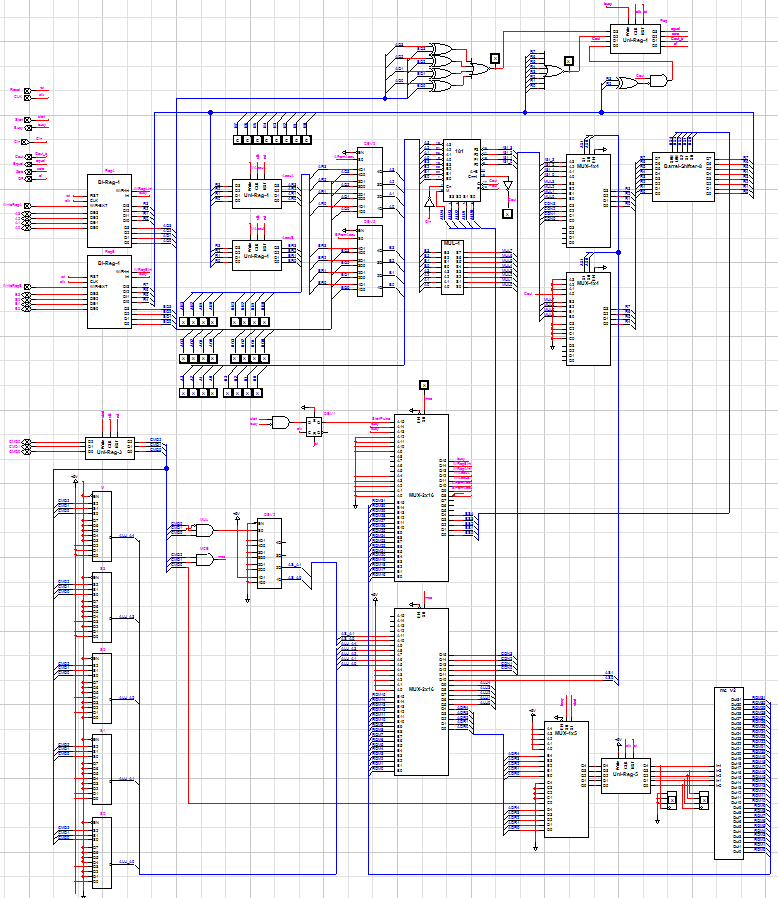
\includegraphics[width=\textwidth]{inneresBlockschaltbild}
			\label{inneresBlockschaltbild}
			\caption{Inneres Blockschaltbild}
		\end{center}
	\end{figure}
	
	\begin{figure}[htbp]
		\begin{center}
			\includegraphics[width=\textwidth]{eingaenge_auswahlregister}
			\label{eingaenge_auswahlregister}
			\caption{Ein-/Ausgänge und Accumulatorregister}
		\end{center}
	\end{figure}
	
	\begin{figure}[htbp]
		\begin{center}
			\includegraphics[]{CMD_ALUbefehle}
			\label{CMD_ALUbefehle}
			\caption{Befehlscodierung}
		\end{center}
	\end{figure}
	
	\begin{figure}[htbp]
		\begin{center}
			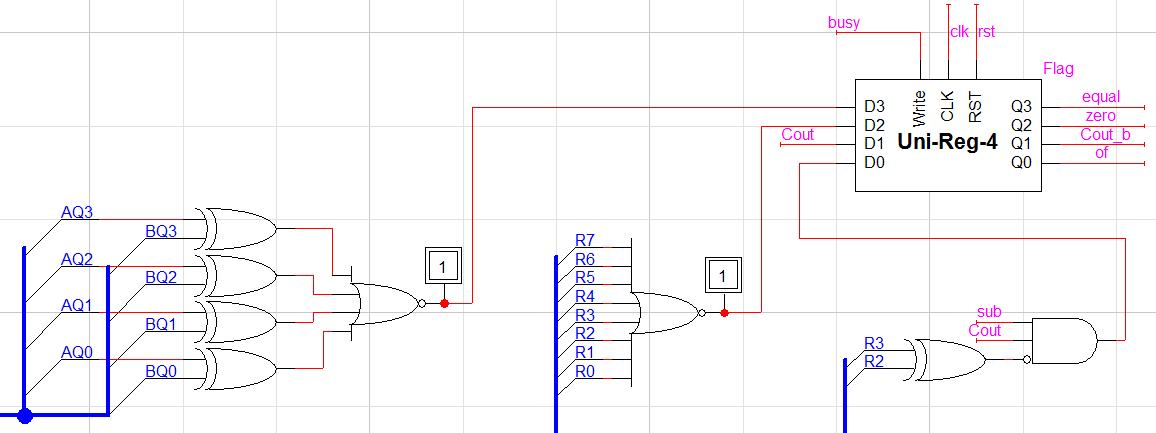
\includegraphics[width=\textwidth]{flagregister}
			\label{flagregister}
			\caption{Bestimmung der Flags}
		\end{center}
	\end{figure}
	
\end{document}